%%%%%%%%%%%%%%%%%%%%%%%%%%%%%%%%%%%%%%%%%%%%%%%%%%%%%%%%%%%%%%%%%%%%%%%%%%%%%%%%
%2345678901234567890123456789012345678901234567890123456789012345678901234567890
%        1         2         3         4         5         6         7         8

%\documentclass[letterpaper, 10 pt, conference]{ieeeconf}  % Comment this line out if you need a4paper

\documentclass[a4paper, 10pt, conference]{ieeeconf}      % Use this line for a4 paper

\IEEEoverridecommandlockouts                              % This command is only needed if 
                                                          % you want to use the \thanks command

\overrideIEEEmargins                                      % Needed to meet printer requirements.

\usepackage{xcolor}
\newcommand\coltxt[2]{\textbf{\textcolor{#1}{(#2)}}}
\newcommand\msm[1]{\coltxt{blue}{MSM:#1}}
\newcommand\dk[1]{\coltxt{green}{DK:#1}}
\newcommand\ds[1]{\coltxt{red}{DS:#1}}

%In case you encounter the following error:
%Error 1010 The PDF file may be corrupt (unable to open PDF file) OR
%Error 1000 An error occurred while parsing a contents stream. Unable to analyze the PDF file.
%This is a known problem with pdfLaTeX conversion filter. The file cannot be opened with acrobat reader
%Please use one of the alternatives below to circumvent this error by uncommenting one or the other
%\pdfobjcompresslevel=0
%\pdfminorversion=4

% See the \addtolength command later in the file to balance the column lengths
% on the last page of the document

% The following packages can be found on http:\\www.ctan.org
\usepackage{graphicx} % for pdf, bitmapped graphics files
\usepackage{epsfig} % for postscript graphics files
\usepackage{mathptmx} % assumes new font selection scheme installed
\usepackage{times} % assumes new font selection scheme installed
\usepackage{amsmath} % assumes amsmath package installed
\usepackage{amssymb}  % assumes amsmath package installed
\usepackage{subcaption}

\title{\LARGE \bf
Compariing SLAM performance under varying simulated environmental conditions in Unity-ROS(Robot Operating System) Simulator for Space Applications(URSSA)
}


\author{Midhun S. Menon$^{1}$ and Daniel Koris$^{2}$ and Daniel Szafir$^{2,3}$ and Jack Burns$^{1}$% <-this % stops a space
\thanks{*This work is directly supported by the NASA Solar System Exploration Research Virtual Institute cooperative agreement 80ARC017M0006.}% <-this % stops a space
\thanks{$^{1}$Center for Astrophysics and Space Astronomy, University of Colorado Boulder}%
\thanks{$^{2}$Department of Computer Science, University of Colorado, Boulder}%
\thanks{$^{3}$ATLAS Institute, University of Colorado, Boulder}%
}


\begin{document}

\twocolumn[{%
\renewcommand\twocolumn[1][]{#1}%

\maketitle

%\begin{figure*}[h]
\begin{center}
   \centering
    \includegraphics[width=\textwidth]{Figures/teaserfig.pdf}
     \vspace{-2em}
    \captionof{figure}{We present a test-bed setup for evaluating vision-based navigation for lunar operations. (A) Virtual lunar topography within the simulation testbed with synthetic terrain and accurate photometric responses modeled after the surface of the moon. (B)  The MER 1 rover model used in our case study simulation. (C) MER 1 camera view of the Opposition Surge}
    \label{teaserfig}
\end{center}
}]

%\maketitle
\thispagestyle{empty}
\pagestyle{empty}


%%%%%%%%%%%%%%%%%%%%%%%%%%%%%%%%%%%%%%%%%%%%%%%%%%%%%%%%%%%%%%%%%%%%%%%%%%%%%%%%
\begin{abstract}
Robots are critical components for space exploration. They help offset safety risks taken by human astronauts, aid in precursor mission tasks prior to manned missions, provide critical on-mission, and post-hoc support. However, designing robotic systems to navigate, map and localize in hostile and unknown extraterrestrial worlds remains open challenge. The primary reason is that testing environments for semi-autonomous agents that will produce robust performance are incredibly challenging to create. To address this issue, we present the Unity3D - ROS (Robot Operating System) Simulator for Space Applications (URSSA) and demonstrate how lighting conditions affect the performance of a single Visual Intertial Odometry (VIO) Simultaneous Localization And Mapping (SLAM) algorithms on lunar surface. The test architecture, agent modeling, rationale for test cases, and generation of ground truth data is discussed. Paper concludes with results from simulations comparing the lighting conditions and discusses on failure reasons and potential directions for improving algorithms for better applicability in such environments. We believe such a comparative study can give vital pointers for future research directions and help accelerate development of specific algorithms for SLAM in extra terrestrial environments.

\end{abstract}


%%%%%%%%%%%%%%%%%%%%%%%%%%%%%%%%%%%%%%%%%%%%%%%%%%%%%%%%%%%%%%%%%%%%%%%%%%%%%%%%
\section{INTRODUCTION}

The last decade has seen major space faring nations chart out focused plans for deep space exploration starting with the moon. The Artemis I\cite{sundahl2020setting},  Chang'e-4 mission\cite{jia2018scientific} and Chandrayaan-2\cite{sundararajan2018overview} are some of the ongoing and completed precursor missions to put human explorers on lunar surface. These missions have robotic systems onboard to do remote investigation, survey, and data collection of the lunar surface. The follow-up to all of these missions have an increasing dependence on ground based robotic systems. Wheeled rovers are the most commonly used platform for planetary surface mobility. To date, they have been used for surface exploration, mapping, and scientific investigation. However, future missions call for advanced operations including periodic monitoring of geo-spatially distributed scientific assets, remote assembly, and In-Situ Resource Utilization(ISRU)\cite{green2019situ} tasks. The cornerstone for all of these tasks is navigation, mapping, and localization capabilities over large ranges. It is even more vital in ISRU tasks which require advanced manipulation and dexterity capabilities. More importantly, these algorithms need to be tested under a rich and varying environment to make sure they perform reliably. In this paper, the focus is demonstrating our test-bad for algorithms for navigation, mapping, and localization. Currently, the space robotics community relies on mission analogs for evaluation and testing of such on-board algorithms. These operations are carried out on Earth in a mock environments of the true mission. However, analogs are incapable of simulating certain critical, unique, and finer aspects of the extraplanetary environment (e.g., gravity, photometric anomalies, etc.) which impacts testing efficacy. As an example, visual artifacts present in a target environment but not simulated in a mission analog may artificially inflate expectations and over-estimate algorithm performance during testing. In a similar vein, locating a matching topography for a mission analog on Earth can also prove an increasing challenge as the geological processes governing surface formation and evolution will differ entirely in most cases.    

In this research, we wish to address the problem of designing virtual analogs for extra-terrestrial environments within a multiphysics framework for advancing research in algorithms that govern low-level autonomy and support interactive trade-offs between various levels of supervisory control. Furthermore, such virtual environments may enable future explorations into the design of new interfaces that support ground control and/or astronaut operation of surface robots from orbital stations. We believe these interfaces will significantly improve critical space exploration missions. 
\section{Current Work}
\begin{figure*}[t]
      \centering
        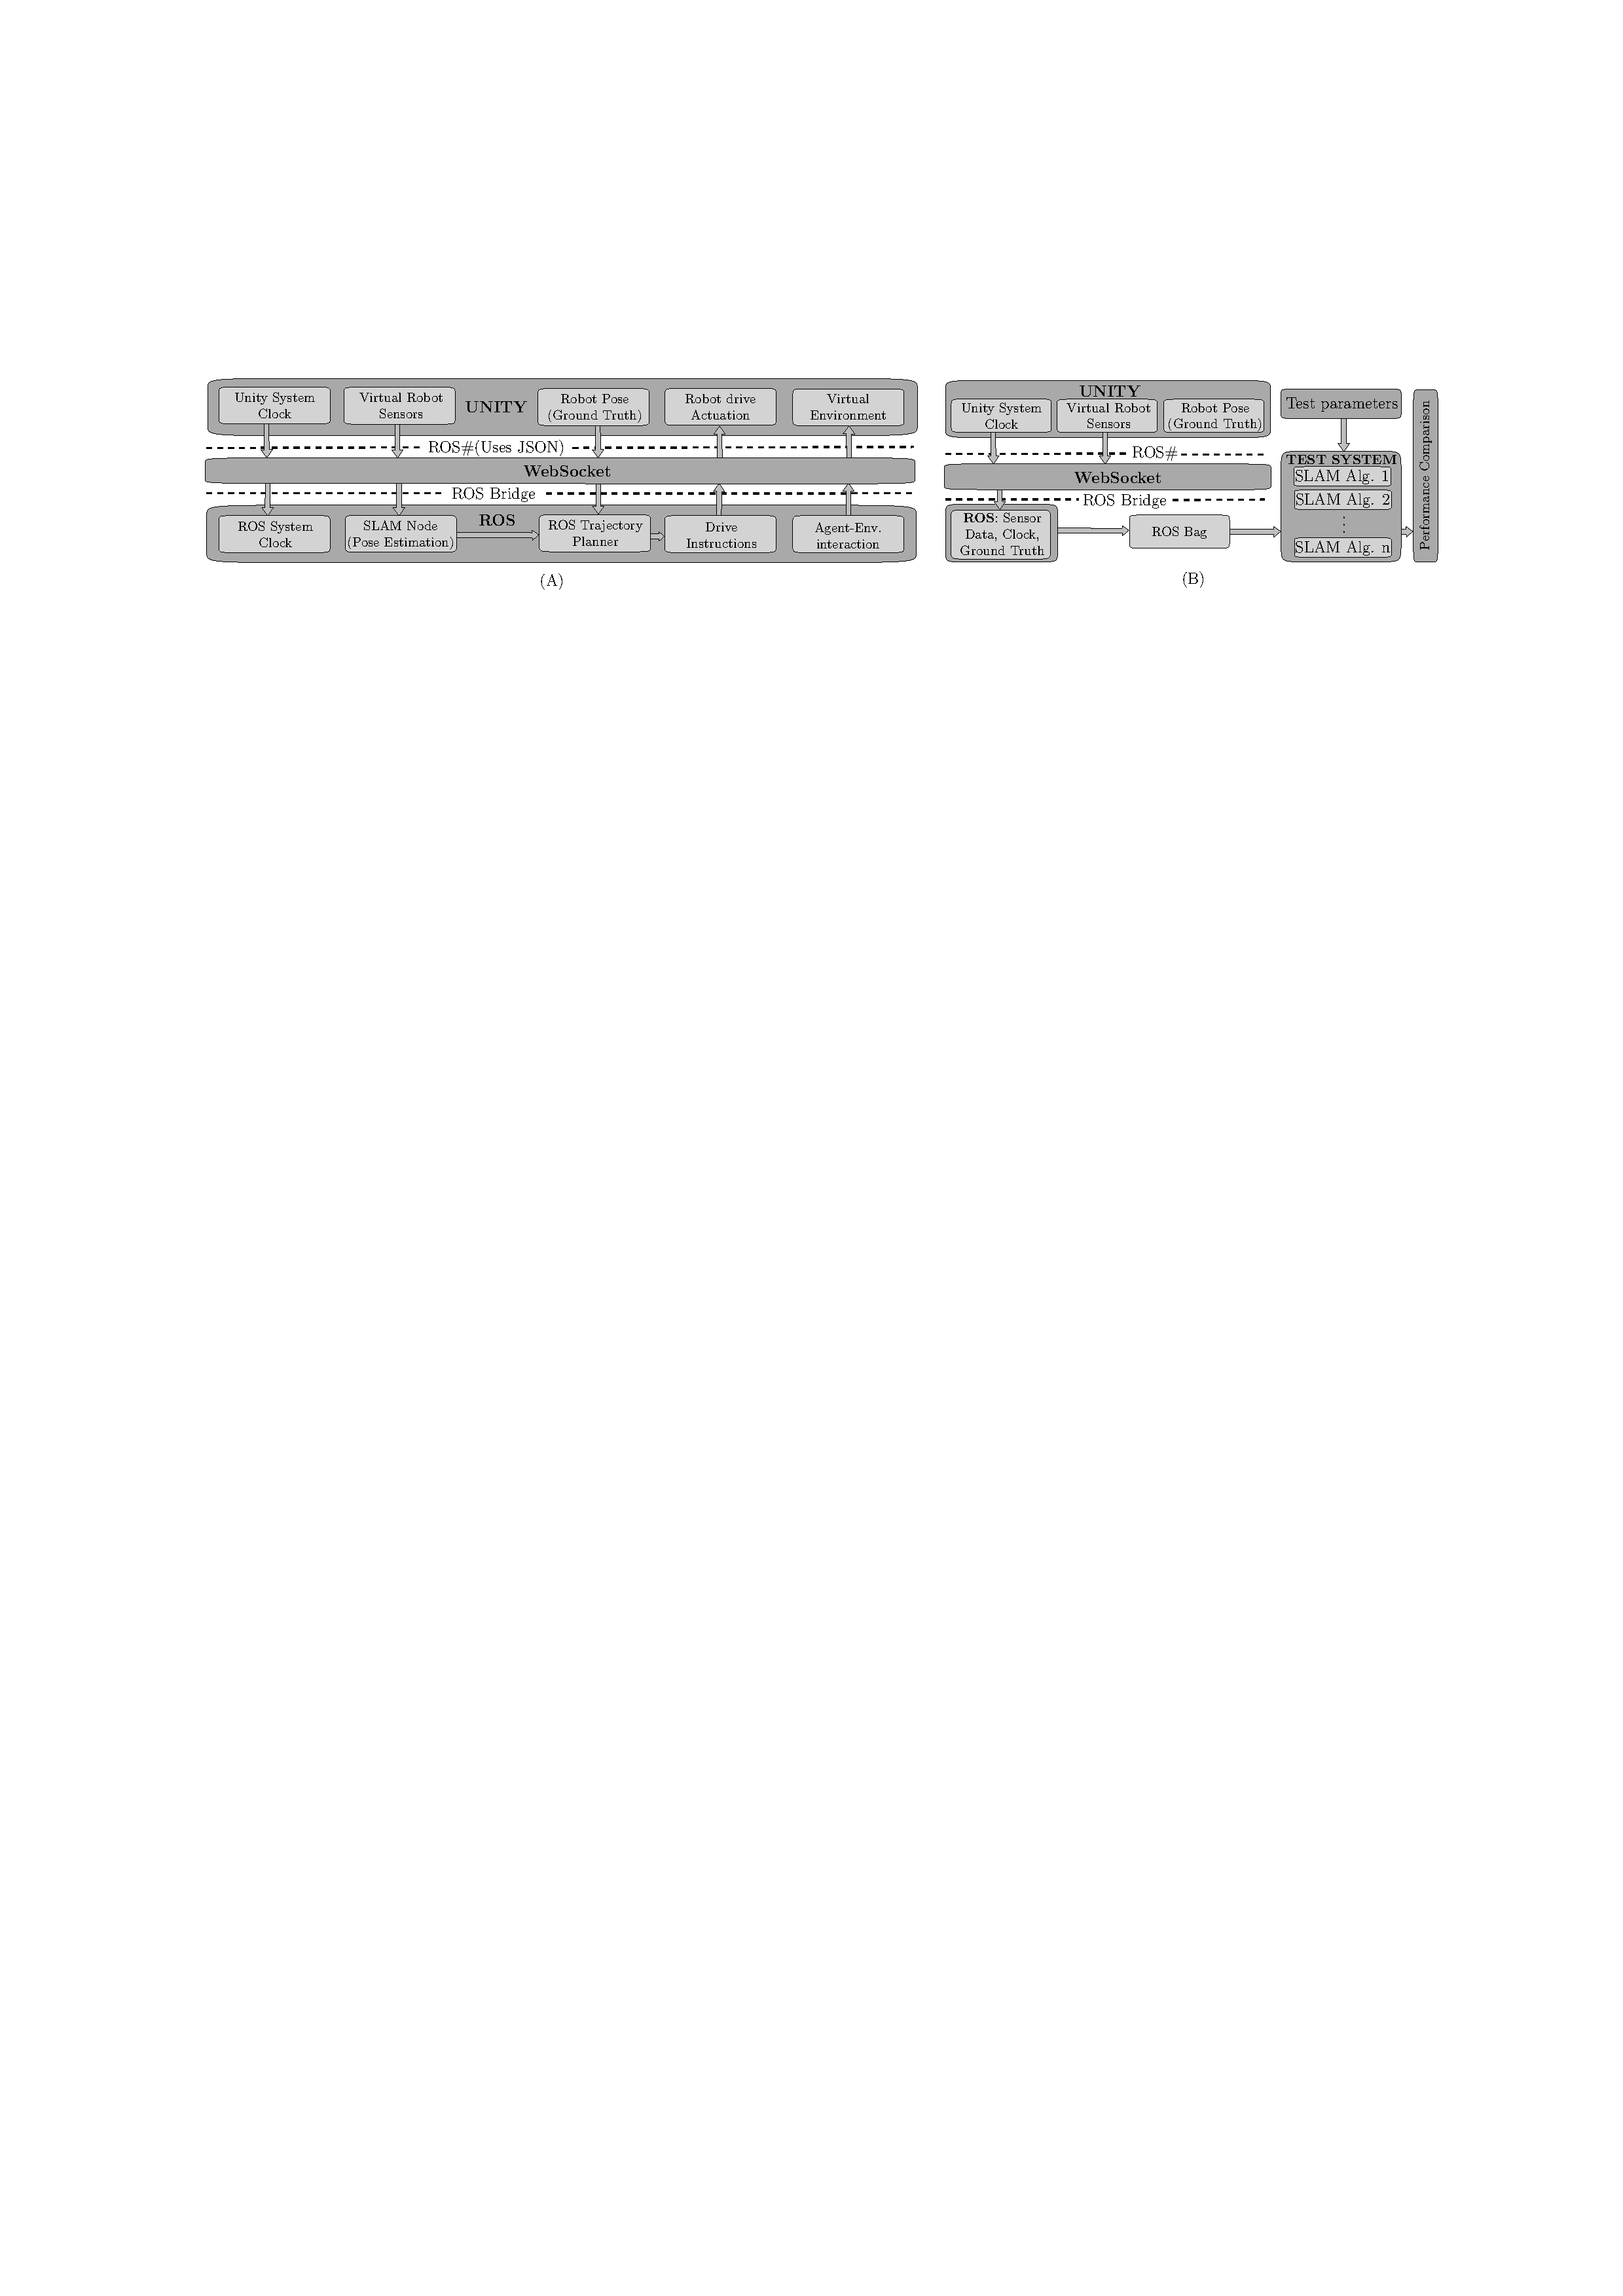
\includegraphics[width=1.0\textwidth]{Figures/sysarch_test_diag.pdf}
      \caption{(A) URSSA system diagram detailing our modular architecture for bidirectional Unity--ROS communication. (B) Test System architecture}
      \vspace{-1em}
      \label{flowchart}
\end{figure*}
Virtual terrain and environments have been in use in the modeling-simulation and computer graphics community for many years. One of the earliest applications of virtual terrain was to model terrain wheel interactions( \cite{yang2007realistic,yang2008virtual,ding2008design,gao2012virtual}). In \cite{andreev2018creating}, virtual environments are used as a training ground for space tasks and mission operations. However, both these applications were limited in scope by only modeling the topography of the terrain. The first applications that had accurate photometric models were visualizations for celestial bodies(\cite{van2011investigation,wright2011preparing, jensen2001physically}) and for investigating perceptual errors made by human beings when inferring the scale and distance of extra-terrestrial environments\cite{oravetz2011slope}. More recently, a commercially available software platform called Planet and Asteroid Natural Scene Generation Utility(PANGU) uses accurate photometric and optical modeling  to create high fidelity simulation of terrains and Entry-Descent-Landing(EDL) simulations(\cite{dunstan2018pangu,martin2019planetary}). However, it is a highly specific software meant only for visualization and the best achievable frame rates are less than 10Hz. 

To the best of our knowledge, the only other framework for simulating the rover-environment interaction is developed inhouse by NASA\cite{allan2019planetary} for moon. However, it has been designed for high-fidelity simulation of lunar environment vision-based navigation algorithms and are limited in scope, scalability and their ability to provide perceptually real-time simulation. In addition, other frameworks are mostly based on classic simulation platform called Gazebo\cite{koenig2004design}, which is not always as efficient, realistic, or scalable as modern engines such as Unity (\cite{engine2008unity, konrad2019simulation}). 

This is the reason for simulators becoming increasingly based on frameworks like ROS\cite{quigley2009ros} and Unity(\cite{babaians2018ros2unity3d,bischoffm_2019_06}). Hence, in this paper, in-house developed simulation framework Unity-ROS Simulator for Space Applications(URSSA)\cite{msm2020rss}\ds{How to cite the RSS paper?} is used(Fig. \ref{teaserfig}), that leverages the Unity game engine as a virtual environment simulator to take advantage of its advanced rendering pipeline, support for reliable physics engines and scalable memory management capabilities. ROS is used as the framework to model the autonomous/semi-autonomous robotic systems interacting with the virtual world in Unity. We demonstrate the comparative testing of three popular Visual and/or Intertial Odometry (VIO)\cite{roumeliotis2002augmenting} Simultaneous Localization And Mapping (SLAM)\cite{durrant1996localization} algorithms for surface exploration of moon. Only visual and inertial sensing modalities have been considered here as these are the ubiquitous sensors reliably flight tested and proven with minimal mass penalties on multiple missions to date by space agencies across the world. However, it may be noted that URSSA has no such restrictions.

\section{Simulator model}
The simulator architecture is shown in Fig.~\ref{flowchart} and consists of three main components. Unity is used for simulating the environment, topography, photometry, rover dynamics and terrain interaction. The second main component is ROS and it is used to simulate the agent behaviour, which essentially takes in the cognitive information of the environment through the simulated sensors, and generates appropriate inferences(SLAM) and actions on how to interact with the environment(path planning). These two independent components are coupled through a communication framework called ROS\#(\cite{bischoffm_2019_06}), which also takes care of time synchronization and guarantees across the components. The details of the modelling are in \cite{msm2020rss}. The following sections give a brief overview each of these components.
\begin{figure*}[t]
      \centering
        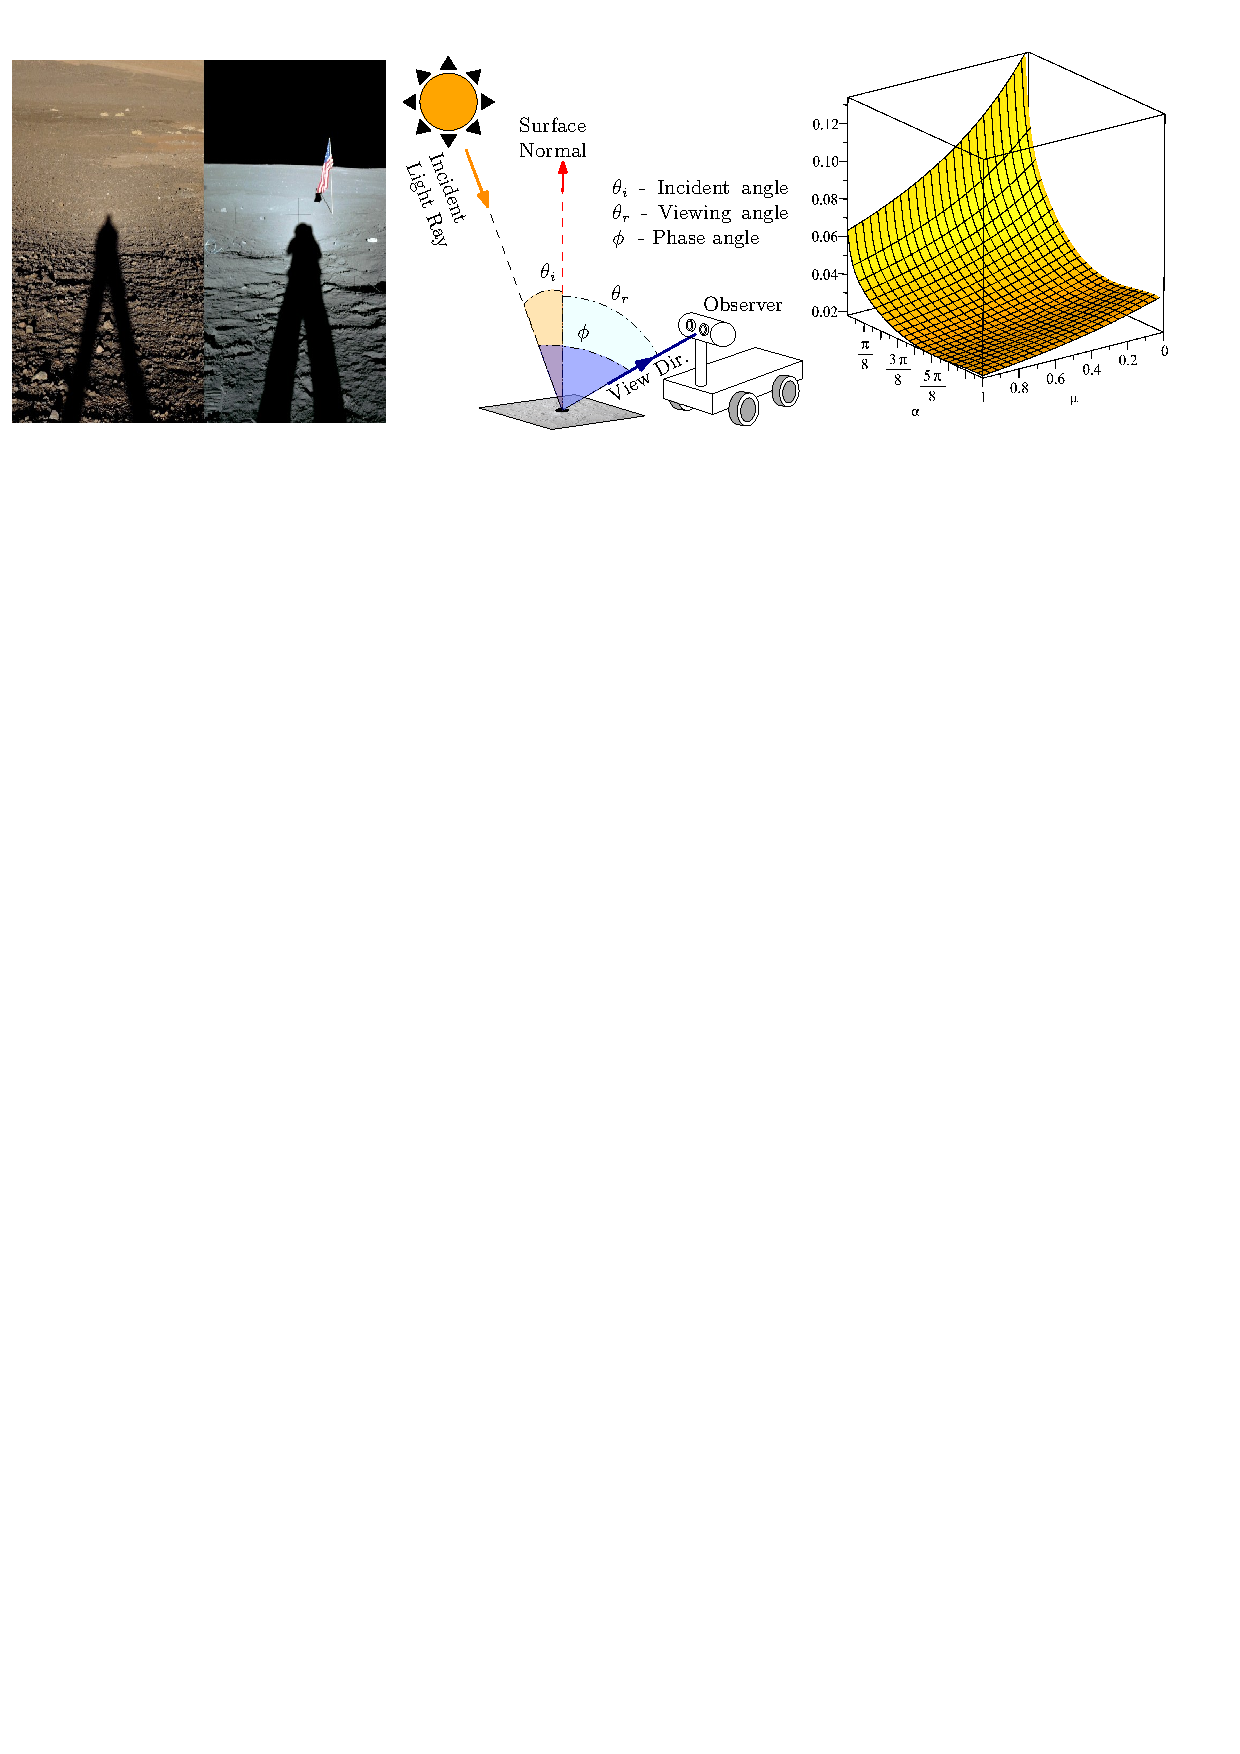
\includegraphics[width=0.85\textwidth]{Figures/brdf_mod_iros.pdf}
      \caption{(A)Comparig similar images taken on earth(left, Atacama desert and moon(right, Apollo 12), Opposition Surge is visible in brightening aroung head shadow Image credit:Molaro/NASA (B)Variables in a BRDF (C)Hapke BRDF plot}
      \vspace{-1em}
      \label{osbrdf}
\end{figure*}
\subsection{Environment model(Unity)}
The virtual environment is modeled as multiple interacting sub-systems inside Unity environment.
\subsubsection{Topographic Model}
The lunar topography is simulated using high-resolution synthetic terrain modeled on actual lunar surface data from Lunar Reconnaissance Orbiter(LRO)-Narrow Angle Camera(NAC) Digital Terrain Models(DTM) which are available to a resolution of 0.5m(at best). Sub-millimeter super-resolved terrain is generated from these DTMs using observed lunar surface roughness parameters(\cite{manned1971analysis,rowan1971lunar}), crater distributions(\cite{neukum1975study,heiken1991lunar}) and boulder distributions \cite{watkins2018boulder} from the Apollo missions to generate physically realistic terrain by fractal expansion algorithms. Rocks of envelope diameters in range of 0.5m--2.0m have also been procedurally generated and uniformly distributed on the terrain as these are not captured by LRO-NAC DTM in its resolution limits(Refer Fig.~\ref{teaserfig}(A,B)).
\subsubsection{Photometric Model}
Custom shaders are developed based on Hapke photometric model\cite{hapke2012theory} to simulate the photometric response of moon called Opposition Surge(OS)\cite{gehrels1964wavelength}(Fig.~\ref{osbrdf}(A)), a specific behaviour exhibited by moon at low phase angles which induces visual artefacts like glare, lens flares and sensor saturation in optical imaging systems. Such artefacts can drastically affect mapping algorithms and perception-aided planners \cite{otsu2017look}. The Hapke Bidirectional Reflectance Distribution Function(BRDF)(Fig.~\ref{osbrdf}(C)) is implemented in the Unity Physically Based Rendering(PBR) pipeline\cite{pranckevivcius2014physically} and the parameters for the same are derived from lunar parameter maps\cite{sato2014resolved}. The variables in the BRDF are the incident angle $\theta_i$, the reflected angle $\theta_r$ and the phase angle $\phi$(Fig.~\ref{osbrdf}(B)). The plot of the Hapke BRDF is shown in Fig.~\ref{osbrdf}(C), which shows the OS when the phase angle approaches zero.
\subsubsection{Rover Mechanical Model}
The rover is modeled as a multi-body system based off the design of Mars Exploration Rover(MER). The rover geometry has been modeled inside Unity(Fig.~\ref{teaserfig}(C)) along with a stereo camera pair at the mast head and Inertial Measurement Unit(IMU) placed on the body. Every attempt is made to match the model rover design and parameters to the MER\cite{crisp2003mars,maki2003mars}. However, the rocker-bogie suspension stiffness/damping parameters and the wheel masses have been tuned to minimize disturbances due to terrain irregularities on the rover body. Thus the suspension in-effect acts as a mechanical low-pass filter to terrain disturbances and also helps guarantee minium three point contact at all times. The six independently powered wheels are distributed as three pairs - front, middle and back. Of these, the front and back pairs act as steering wheels. Moreover, rover left and right rockers counter rotate actively to self balance the rover when moving over obstacles, as implemented in MER.
\subsubsection{Rover Sensor Models}
An exploratory rover operating in an unknown/partially known enviroment will likely have multiple sensors that collect data across various modalities \cite{borenstein1997mobile,ruocco2013robot}, ranging from hyper-spectral optical imagers (visible, infrared, ultraviolet, radio-spectrum etc.), haptic sensors, 3D ranging sensors (structured light sensors, stereo imagers, LIDARs etc.), odometry sensors, inertial sensors, etc. While the framework theoretically enables simulating any of these sensor modalities, two types of sensors are used in this paper : visible spectrum cameras (monocular and binocular)  and Inertial Measurement Unit (IMU), the reasons being that these are the most reliable and least space/mass penalizing sensors on extra-terrestrial mobility platforms. 

The IMU is modeled with based on sensor models suggested by \cite{savage1998strapdown1} and \cite{savage1998strapdown2} and elucidated in \cite{titterton2004strapdown}. In short, the ground truth pose data of the frame is corrupted with noise from double integration of bias, scale factor uncertainties, and Additive White Gaussian Noise (AWGN) on angular rates (gyros) and accelerations (accelerometers).

The imaging sensor is modeled as a pinhole camera with radial distortion. The camera parameters are kept at the same values as  the MER mast camera stereo pair(refer table in p4,\cite{maki2003mars}).

\subsubsection{Wheel-Terrain Interaction Model}
The wheels on the rover have been modeled as ellipsoids so as to simplify collider computations. Wheeled vehicles on lunar regolith experiences skid, slip and sinkage\cite{ding2009slip}. There are various traction models in literature to predict the contact forces at the wheel soil interface based on continuum  methods(\cite{bekker1964mechanics,wong1967behaviour,ding2015interaction}), Discrete Element Models(\cite{yoshida2003terramechanics,jeong2019development,rodriguez2019high,jiang2018experimental,jeong2019development}) and empirical models(\cite{huang2019sinkage,wong2012predicting}).  However, as a first level simplification, in this paper, slip alone is considered with Coulomb dry friction model, wherein traction force is proportional to the normal reaction at the wheel-soil interface. Subsequent studies will incorporate some of the more advanced traction models mentioned above.
\subsection{Agent Model(ROS)}
The virtual robotic agents which are the processing and decision making portion of the robot is implemented as nodes in ROS. The SLAM algorithm runs as a ROS node, which estimates the robot's pose and trajectory. A ROSbridge node\cite{crick2017rosbridge} acts as the modem between ROS and Unity. ROSbridge is used to stream sensor data from Unity  to ROS nodes  and send drive commands ROS to Unity.  
\subsection{Communication Framework(ROS\#)}
The ROS\# framework is used to enable communication between Unity and ROS. The framework enables Unity to publish and subscribe to topics on  a ROS nodes by encoding/decoding information using JSON format and communicating through websockets. 
\subsubsection{Time Synchronization}
Right  out-of-the-box, the system does not have time synchronization as the time-scales vary between ROS and Unity, due to which time flows at different rates. As the publisher-subscriber model is asynchronous, time needs to be explicitly synchronized as all estimates are time stamped. Our architecture leverages a feature of ROS to coordinate timing across its distributed architecture as a properly designed ROS node may use all internal ROS timing mechanisms rather than machine-level timing mechanisms. These ROS timing mechanisms can be driven by an external synchronizing entity. In our case, since Unity is providing the simulation environment and is seen as the potential timing bottle-neck in the system, we publish a topic from Unity to drive the ROS internal timings. Since all data is time-stamped on both ends, and Unity is the singular clock generating timestamps, our framework is robust in terms of distributed temporal synchronization; in other words, if there is a delay on the Unity side, that delay will be propagated in the ROS system (although we note in our testing to-date, the system runs in perceptually real time).
\subsubsection{Real Time compliance}
If the simulator is to plugin to an external agent with independent clock, the combined system will loose time-synchronization. A typical scenario is the case where the simulator is interfaced with a independent SLAM algorithm running its own clock internally, in which case estimation results will be wrongly time stamped causing accumulated error over time. In order to avoid this, the WebRTC architecture\cite{loreto2014real} is implemented for the Unity websocket communication. The WebRTC is a Real-Time Compliant websocket communication architecture with hard-realtime guarantees, thereby helping to mitigate the timing issue  and making the simulator robust. 
\subsubsection{Fixed Update}
The \textit{FixedUpdate} method is used for the physics calculations in Unity by which fidelity of the physics calculations are guaranteed at a fixed rate independent of the rendering frame rate. This helps make sure that physics computations are not skipped when the rendering frame rate gets throttled, making the simulation more robust to numerical errors and instabilities from large integration steps.
\section{Test System}
The objective of this test system is to evaluate and compare effect/sensitivity of environmental parameters on the performance of SLAM algorithms on extra-terrestrial planetary bodies. Data is recorded over preset trajectories on the terrain using rosbags and fed as input to the SLAM algorithm, who then estimate the pose based on these inputs. Due to the probabilistic nature of many SLAM algorithms, statistical measures over multiple iterations of the same trajectory are generated and reported for performance evaluation(refer Fig.~\ref{flowchart}(B)).
The main variables in this model are (a) Sun-Camera geometry (b) Shader Hapke coefficients (c) Path type.
\subsection{Sun-Camera Geometry}
To study performance under varying extremes of sun-camera geometry, two positions of sun's elevation-$20^\circ$(dawn/dusk) and $90^\circ$(noon) are chosen. And at each of these elevations,  three azimuths(with respect to rover camera) are tested-$0^\circ$(anti), $90^\circ$(cross) and $180^\circ$(pro). These conditions together simulate the solar geometry extremes over a lunar day and evaluate performance.
\subsection{Shader Hapke coefficients}
To evaluate algorithm performance under varying shader backscatter conditions, four test cases are proposed - two high albedo(adversarial), one nominal and two low albedo(adversarial) shader parameter set. The albedo and backscatter coefficients are modified here to generate the various test environments. This will help evaluate performance and sensitivity to shader parameters and perturbations.
\subsection{Path type}
For comparing performance under different types of trajectory shapes, the algorithms have to be run with two types of trajectories - straight and circular. This helps verify the performance of the algorithms when making gradual turns and also to check for loop-closure.

Weeding out the duplicates in above mentioned test case set, the system has a total of 40 test cases.
\section{Simulation }
For this case study, we leveraged the modular architecture of URSSA to run a simulation using desktop PCs to distribute the compute load of virtual environment rendering and running SLAM. One machine (Intel 3.6 GHz processor, 32 GB RAM, NVIDIA GeForce RTX 2080 8 GB graphics card) ran the Unity environment simulation using Microsoft Windows 10 while the other (Intel 4 GHz processor, 8 GB RAM, NVIDIA GeForce GTX 1070 8 GB graphics card) performed the back-end SLAM estimation and robotic control using ROS Kinetic on Ubuntu 16.04. In the virtual lunar environment, the only source of illumination was sunlight, which was modeled as a directional white source (R:255,G:255,B:255). The virtual $1km\times 1km$ lunar terrain was modeled with a resolution of 0.5mm to ensure it has enough fidelity even when viewed from a height of 0.8m--1.0m (i.e., the typical height of a mast camera for a micro-rover).
The basline is chosen as the condition at lunar dawn with sun elevation angle of $20^\circ$, the typical solar elevation angle when solar generation rate breaks even with nominal power consumption for a micro rover. The solar azimuth for the baseline case is chosen as $90^\circ$ which is the solar azimuth when you make a polar movement during lunar dawn or lunar dusk (can be $180^\circ$ also) on moon starting from equator. The camera parameters including the intrinsics and stereo baseline is calibrated for this reference test case. The rover is allowed to traverse at constant average velocity of 0.4 m/s for 100 seconds on the straight line trajectory and 0.3 m/s for 110 seconds on a circular trajectory with a steering angle held at a constant $10^\circ$ (longer time for the trajectory is given to complete the full circle). Please note that this velocity is higher than the typical extra-terrestrial rover travesal velocities of 0.05m/s, the reason for this being that we wanted to make sure that the test trajectories were long enough to allow for sufficient error accumulation so as to be observed. Also, in this case-study, only representative runs of each test case have been implemented, though in general multiple runs have to be done and the expected values are to be reported. The trajectories are chosen inside a crater in the terrain so that a feature rich environment is available for the SLAM to get better estimates (though this will be relaxed in future iterations).

\section{Results and Discussion}
\subsection{Straight Path}
For the straight path, the main errors to be quantified are the drifts along X, Y and Z directions. On straight path, an approximate traverse distance of 34m was carried out. 
\subsection{Circular Path}
\section{Conclusion}
To be Done.

\bibliographystyle{IEEEtran}
\bibliography{IEEEabrv,refs}


\end{document}
